\documentclass[a4paper,10pt,reqno]{amsart}

\usepackage[utf8]{inputenc}
\usepackage[foot]{amsaddr}
\usepackage{amsmath,amsfonts,amssymb,amsthm,mathrsfs,bm}
\usepackage[margin=0.95in]{geometry}
\usepackage{color}
\usepackage[dvipsnames]{xcolor}

\usepackage{etoolbox}

% Modifications to amsart ToC-related macros...
\makeatletter
\let\old@tocline\@tocline
\let\section@tocline\@tocline
% Insert a dotted ToC-line for \subsection and \subsubsection only
\newcommand{\subsection@dotsep}{4.5}
\newcommand{\subsubsection@dotsep}{4.5}
\patchcmd{\@tocline}
  {\hfil}
  {\nobreak
     \leaders\hbox{$\m@th
        \mkern \subsection@dotsep mu\hbox{.}\mkern \subsection@dotsep mu$}\hfill
     \nobreak}{}{}
\let\subsection@tocline\@tocline
\let\@tocline\old@tocline

\patchcmd{\@tocline}
  {\hfil}
  {\nobreak
     \leaders\hbox{$\m@th
        \mkern \subsubsection@dotsep mu\hbox{.}\mkern \subsubsection@dotsep mu$}\hfill
     \nobreak}{}{}
\let\subsubsection@tocline\@tocline
\let\@tocline\old@tocline

\let\old@l@subsection\l@subsection
\let\old@l@subsubsection\l@subsubsection

\def\@tocwriteb#1#2#3{%
  \begingroup
    \@xp\def\csname #2@tocline\endcsname##1##2##3##4##5##6{%
      \ifnum##1>\c@tocdepth
      \else \sbox\z@{##5\let\indentlabel\@tochangmeasure##6}\fi}%
    \csname l@#2\endcsname{#1{\csname#2name\endcsname}{\@secnumber}{}}%
  \endgroup
  \addcontentsline{toc}{#2}%
    {\protect#1{\csname#2name\endcsname}{\@secnumber}{#3}}}%

% Handle section-specific indentation and number width of ToC-related entries
\newlength{\@tocsectionindent}
\newlength{\@tocsubsectionindent}
\newlength{\@tocsubsubsectionindent}
\newlength{\@tocsectionnumwidth}
\newlength{\@tocsubsectionnumwidth}
\newlength{\@tocsubsubsectionnumwidth}
\newcommand{\settocsectionnumwidth}[1]{\setlength{\@tocsectionnumwidth}{#1}}
\newcommand{\settocsubsectionnumwidth}[1]{\setlength{\@tocsubsectionnumwidth}{#1}}
\newcommand{\settocsubsubsectionnumwidth}[1]{\setlength{\@tocsubsubsectionnumwidth}{#1}}
\newcommand{\settocsectionindent}[1]{\setlength{\@tocsectionindent}{#1}}
\newcommand{\settocsubsectionindent}[1]{\setlength{\@tocsubsectionindent}{#1}}
\newcommand{\settocsubsubsectionindent}[1]{\setlength{\@tocsubsubsectionindent}{#1}}

% Handle section-specific formatting and vertical skip of ToC-related entries
% \@tocline{<level>}{<vspace>}{<indent>}{<numberwidth>}{<extra>}{<text>}{<pagenum>}
\renewcommand{\l@section}{\section@tocline{1}{\@tocsectionvskip}{\@tocsectionindent}{}{\@tocsectionformat}}%
\renewcommand{\l@subsection}{\subsection@tocline{1}{\@tocsubsectionvskip}{\@tocsubsectionindent}{}{\@tocsubsectionformat}}%
\renewcommand{\l@subsubsection}{\subsubsection@tocline{1}{\@tocsubsubsectionvskip}{\@tocsubsubsectionindent}{}{\@tocsubsubsectionformat}}%
\newcommand{\@tocsectionformat}{}
\newcommand{\@tocsubsectionformat}{}
\newcommand{\@tocsubsubsectionformat}{}
\expandafter\def\csname toc@1format\endcsname{\@tocsectionformat}
\expandafter\def\csname toc@2format\endcsname{\@tocsubsectionformat}
\expandafter\def\csname toc@3format\endcsname{\@tocsubsubsectionformat}
\newcommand{\settocsectionformat}[1]{\renewcommand{\@tocsectionformat}{#1}}
\newcommand{\settocsubsectionformat}[1]{\renewcommand{\@tocsubsectionformat}{#1}}
\newcommand{\settocsubsubsectionformat}[1]{\renewcommand{\@tocsubsubsectionformat}{#1}}
\newlength{\@tocsectionvskip}
\newcommand{\settocsectionvskip}[1]{\setlength{\@tocsectionvskip}{#1}}
\newlength{\@tocsubsectionvskip}
\newcommand{\settocsubsectionvskip}[1]{\setlength{\@tocsubsectionvskip}{#1}}
\newlength{\@tocsubsubsectionvskip}
\newcommand{\settocsubsubsectionvskip}[1]{\setlength{\@tocsubsubsectionvskip}{#1}}

% Adjust section-specific ToC-related macros to have a fixed-width numbering framework
\patchcmd{\tocsection}{\indentlabel}{\makebox[\@tocsectionnumwidth][l]}{}{}
\patchcmd{\tocsubsection}{\indentlabel}{\makebox[\@tocsubsectionnumwidth][l]}{}{}
\patchcmd{\tocsubsubsection}{\indentlabel}{\makebox[\@tocsubsubsectionnumwidth][l]}{}{}

% Allow for section-specific page numbering format of ToC-related entries
\newcommand{\@sectypepnumformat}{}
\renewcommand{\contentsline}[1]{%
  \expandafter\let\expandafter\@sectypepnumformat\csname @toc#1pnumformat\endcsname%
  \csname l@#1\endcsname}
\newcommand{\@tocsectionpnumformat}{}
\newcommand{\@tocsubsectionpnumformat}{}
\newcommand{\@tocsubsubsectionpnumformat}{}
\newcommand{\setsectionpnumformat}[1]{\renewcommand{\@tocsectionpnumformat}{#1}}
\newcommand{\setsubsectionpnumformat}[1]{\renewcommand{\@tocsubsectionpnumformat}{#1}}
\newcommand{\setsubsubsectionpnumformat}[1]{\renewcommand{\@tocsubsubsectionpnumformat}{#1}}
\renewcommand{\@tocpagenum}[1]{%
  \hfill {\mdseries\@sectypepnumformat #1}}

% Small correction to Appendix, since it's still a \section which should be handled differently
\let\oldappendix\appendix
\renewcommand{\appendix}{%
  \leavevmode\oldappendix%
  \addtocontents{toc}{%
    \protect\settowidth{\protect\@tocsectionnumwidth}{\protect\@tocsectionformat\sectionname\space}%
    \protect\addtolength{\protect\@tocsectionnumwidth}{2em}}%
}
\makeatother

% #1 (default is as required)

% #2

% #3
\makeatletter
\settocsectionnumwidth{2em}
\settocsubsectionnumwidth{2.5em}
\settocsubsubsectionnumwidth{3em}
\settocsectionindent{1pc}%
\settocsubsectionindent{\dimexpr\@tocsectionindent+\@tocsectionnumwidth}%
\settocsubsubsectionindent{\dimexpr\@tocsubsectionindent+\@tocsubsectionnumwidth}%
\makeatother

% #4 & #5
\settocsectionvskip{10pt}
\settocsubsectionvskip{0pt}
\settocsubsubsectionvskip{0pt}

% #6 & #7
% See #3

% #8
\renewcommand{\contentsnamefont}{\bfseries\Large}

% #9
\settocsectionformat{\bfseries}
\settocsubsectionformat{\mdseries}
\settocsubsubsectionformat{\mdseries}
\setsectionpnumformat{\bfseries}
\setsubsectionpnumformat{\mdseries}
\setsubsubsectionpnumformat{\mdseries}

% #10
% Insert the following command inside your text where you want the ToC to have a page break
\newcommand{\tocpagebreak}{\leavevmode\addtocontents{toc}{\protect\clearpage}}

% #11
\let\oldtableofcontents\tableofcontents
\renewcommand{\tableofcontents}{%
  \vspace*{-\linespacing}% Default gap to top of CONTENTS is \linespacing.
  \oldtableofcontents}

\usepackage{mathtools,enumerate,mathrsfs,graphicx}
\usepackage{epstopdf}
\usepackage{hyperref}

\usepackage{latexsym}


\definecolor{CommentGreen}{rgb}{0.0,0.4,0.0}
\definecolor{Background}{rgb}{0.9,1.0,0.85}
\definecolor{lrow}{rgb}{0.914,0.918,0.922}
\definecolor{drow}{rgb}{0.725,0.745,0.769}

\usepackage{listings}
\usepackage{textcomp}
\lstloadlanguages{Matlab}%
\lstset{
    language=Matlab,
    upquote=true, frame=single,
    basicstyle=\small\ttfamily,
    backgroundcolor=\color{Background},
    keywordstyle=[1]\color{blue}\bfseries,
    keywordstyle=[2]\color{purple},
    keywordstyle=[3]\color{black}\bfseries,
    identifierstyle=,
    commentstyle=\usefont{T1}{pcr}{m}{sl}\color{CommentGreen}\small,
    stringstyle=\color{purple},
    showstringspaces=false, tabsize=5,
    morekeywords={properties,methods,classdef},
    morekeywords=[2]{handle},
    morecomment=[l][\color{blue}]{...},
    numbers=none, firstnumber=1,
    numberstyle=\tiny\color{blue},
    stepnumber=1, xleftmargin=10pt, xrightmargin=10pt
}

\numberwithin{equation}{section}
\synctex=1

\hypersetup{
    unicode=false, pdftoolbar=true, 
    pdfmenubar=true, pdffitwindow=false, pdfstartview={FitH}, 
    pdftitle={ELE2038 Group 13 Coursework}, pdfauthor={Michael Loughran, Scott McNeilly and Xiaohan Song},
    pdfsubject={ELE2038 Group 13 Coursework}, pdfcreator={Michael Loughran, Scott McNeilly and Xiaohan Song},
    pdfproducer={ELE2038}, pdfnewwindow=true,
    colorlinks=true, linkcolor=red,
    citecolor=blue, filecolor=magenta, urlcolor=cyan
}


% CUSTOM COMMANDS
\renewcommand{\Re}{\mathbf{re}}
\renewcommand{\Im}{\mathbf{im}}
\newcommand{\R}{\mathbb{R}}
\newcommand{\N}{\mathbb{N}}
\newcommand{\C}{\mathbb{C}}
\newcommand{\lap}{\mathscr{L}}
\newcommand{\dd}{\mathrm{d}}
\newcommand{\smallmat}[1]{\left[ \begin{smallmatrix}#1 \end{smallmatrix} \right]}

%opening
\title[ELE2038 Coursework]{ELE2038 Coursework Group 13}
\author{Michael Loughran\vspace{-2mm}}
\author{Scott McNeilly\vspace{-2mm}}
\author{Xiaohan Song\vspace{-2mm}} 

\begin{document}
    \maketitle
    \begin{center}
    \hfill \\
    
\includegraphics[width=0.20\linewidth]{Main/qub logo.jpeg}
    \end{center}

    \tableofcontents
    \section*{Introduction}
In this report, the results of a PID controller that has been designed to control a system that consists of a ball with a metal core on an inclined plane, held by a spring and damper system and attracted by an electromagnet, will be reported and discussed, including the calculations and code used in the process of designing the controller.
The objective for the controller is to hold the ball close to a set point that is 0.5 m down the plane from the top. The controller will need to be BIBO stable, have an offset of zero, and be tuned to avoid large amplitude oscillations and reject disturbances.
\\
The code used for this report can be found here:
\begin{itemize}
  \item \href{https://github.com/40327859/ELE2038-Control-Coursework-Group-13/blob/main/Group13_sympy.ipynb}{Equations and Calculations Code}
  \item \href{https://github.com/40327859/ELE2038-Control-Coursework-Group-13/blob/main/Group13_simulations.ipynb}{Control library and Simulations Code}
\end{itemize}


    \section{Modelling}
\begin{figure}[ht]
    \centering
    \begin{minipage}{0.6\textwidth}
        \centering
        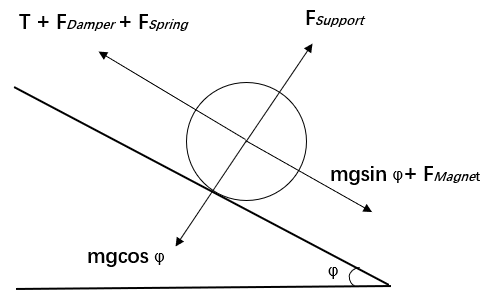
\includegraphics[width=1.20\linewidth]{modelling/Force analysis diagram of the system.png}
        \caption{Force analysis diagram of the system} 
    \end{minipage}
\end{figure}
Modelling involves describing the system, including all forces acting on the system, using mathematics to
allow the system to be analysed. 
\subsection*{Horizontal Forces Equations} \hfill \\
Firstly, we will look at the forces that act horizontally on the which are:

\begin{equation}
    T + F_{\text{Damper}} + F_{\text{Spring}} = mg\sin{\phi} + F_{\text{Magnet}}
\end{equation}
Using newtons second law $F = ma,\  F = m\ddot{\theta} $
\\
\begin{equation}
    m\ddot{x} = mg\sin{\phi} + F_{\text{Magnet}} -T - F_{\text{Damper}} - F_{\text{Spring}}
\end{equation}
\\
Finding T (static friction), using the Torque equation, $Tr = I\ddot{\theta} $ which then if we use the equation for the initial inertia of a sphere which is $I = \frac{2}{5}mr^2$ . Substituting these together, we get:
\begin{equation}
    T = \frac{\frac{2}{5}mr^2}{r}\Ddot{\theta}
\end{equation}
Since $\Ddot{x} = \Ddot{\theta}r, \Ddot{\theta} = \frac{\Ddot{x}}{r}$ we can substitute this into the equation to get:
\begin{equation}
T = \frac{2}{5}\Ddot{x}m
\end{equation}
Finding $F_{\text{Damper}} $, we know from the diagram that:
\begin{equation}
    F_{\text{Damper}} = b\dot{x}
\end{equation}
Finding $F_{\text{Spring}} $, we know from Hooke's law:
\begin{equation}
   F_{\text{Spring}} =  k(x-d)
\end{equation}
From the question, we are told that:
\begin{equation}
    F_{\text{Magnet}} = c\frac{i^2}{y^2}
\end{equation}
By inspection of the diagram, we can see that $y = \delta - x $ thus,
\begin{equation}
    F_{\text{Magnet}} = c\frac{i^2}{(\delta - x)^2}
\end{equation}
Substituting all equations in we get:
\begin{equation}
     mg\sin{\phi} + c\frac{i^2}{(\delta - x)^2} -\frac{2}{5}m\Ddot{x} - b\dot{x} -k(x-d)  = m\Ddot{x} 
\end{equation}
Arranging for $\Ddot{x} $, we get: 
\\ 
\begin{equation}
\Ddot{x} = (\frac{5}{7m})  \left(mg\sin{\phi} + c\frac{i^2}{(\delta - x)^2} - b\dot{x} -k(x-d)  \right)
\end{equation}
\\
\subsection*{Circuit Equations}\hfill \\
Using Kirchhoff's Voltage Law and Ohm's law on the circuit, we obtain the following:
\begin{equation}
v = iR + L\frac{di}{dt}   
\end{equation}
We can take $\frac{di}{dt} = \Dot{i} $ thus,
\\
\begin{equation}
      v = iR +L\Dot{i}  
\end{equation}
Rearranging for $\dot{i} $
\begin{equation}
    \dot{i} = \frac{v - iR}{L}  
\end{equation}
L is given as:
\begin{align*}
    L &= L_0 + L_1e^{-\alpha y^2}\\
    L &= L_0 + L_1e^{-\alpha (\delta - x)^2}
\end{align*}
\subsection*{Combining Equations}\hfill \\
To simplify the calculations, we will put our calculations in terms of $x $:
\begin{align*}
    x_1 &= x
    \\
    x_2 &= \Dot{x} 
    \\
    x_3 &= i
\end{align*}

We can now rewrite all our equations and put them in this form:

\begin{equation}
\begin{bmatrix}
\Dot{x}_1 \\
\Dot{x}_2 \\
\Dot{x}_3
\end{bmatrix} 
=
\begin{bmatrix}
 x_2\\
(\frac{5}{7m})  \left(mg\sin{\phi} + c\frac{x_3^2}{(\delta - x_1)^2} - bx_2 -k(x_1-d)  \right)\\
\frac{v - x_3R}{L_0 + L_1e^{-\alpha (\delta - x_1)^2}}  
\end{bmatrix} 
\end{equation}
    ~\\
\section{Equilibrium Equations}
The equilibrium point of a stable system is the point where the system will return to despite any change of
inputs. This means that by finding a system’s equilibrium point, the stability of the system can be analysed.
\subsection*{Substituting Zero into Derivative Equations}\hfill \\
If we set all the derivatives of our variables to 0 at our equilibrium values, we get:

\begin{align}
    0 &= x_2^{e}\\
    0 &= \frac{5}{7m}  \left(mg\sin{\phi} + c\frac{x_3^{e2}}{(\delta - x_1^{e})^2} -k(x_1^{e}-d) -bx_2^{e}   \right)\\
    0 &= \frac{v^{e} - x_3^{e}R}{L_0 + L_1e^{-\alpha (\delta - x_1^{e})^2}}
\end{align}
\subsection*{Finding Equilibrium Values}
\hfill \\
Since we are told that $x^e_1 = 0.5$ , since it is stationary at this point, we can assume that $x^e_2 = 0$. If we rearrange equation 2.2 we can find the value of $x^e_3 $.
\begin{equation}
    x_3^e = \sqrt{\frac{(kx_1 - kd - mg\sin\phi)(\delta - x_1)^2}{c}}
\end{equation}
If we subsitute our constant values we get $x_3 = 0.707488266645418 $ A.
    
\section{Linearisation} 
Linearisation is used to approximate a linear system from a non-linear system. This linear system can be
found at the system’s equilibrium point. This allows us to analyse the system’s behaviour around the set point
and it is easier to analyse a linear system rather than a non-linear system.
To linearise, we use \texttt{sympy} to determine the partial derivatives of the system dynamics with respect to the states and the input. We define
\begin{equation}
    \phi = \frac{5}{7m}  \left(mg\sin{\phi} + c\frac{x_3^{e2}}{(\delta - x_1^{e})^2} -k(x_1^{e}-d) -bx_2^{e}   \right)
\end{equation}
\subsection*{Partial Derivatives of Phi}
\hfill \\
When we partially derive each equation, we get:
\begin{align}
\left.\frac{\partial \phi}{\partial x_1}\right|_{x_1^e, x_2^e, x_3^e,v^e} ={}& \frac{5 \left(\frac{2 c x_{3}^{2}}{\left(\delta - x_{1}\right)^{3}} - k\right)}{7 m}
\\
\left.\frac{\partial \phi}{\partial x_2}\right|_{x_1^e, x_2^e, x_3^e,v^e} ={}&  - \frac{5 b}{7 m}
\\
\left.\frac{\partial \phi}{\partial x_3}\right|_{x_1^e, x_2^e, x_3^e,v^e} ={}&  \frac{10 c x_{3}}{7 m \left(\delta - x_{1}\right)^{2}}
\\
\end{align}
\subsection*{Partial Derivatives of Psi} \hfill \\
\begin{equation}
    \psi = \frac{v - x_3R}{L_0 + L_1e^{-\alpha (\delta - x_1)^2}}
\end{equation}
When we partially derive each equation, we get:
\begin{align}
\left.\frac{\partial \psi}{\partial x_1}\right|_{x_1^e, x_2^e, x_3^e,v^e} ={}& - \frac{L_{1} \alpha \left(- R x_{3}^e + v\right) e^{- \alpha \left(\delta - x_{1}^e\right)}}{\left(L_{0} + L_{1} e^{- \alpha \left(\delta - x_{1}^e\right)}\right)^{2}}
\\
\left.\frac{\partial \psi}{\partial x_3}\right|_{x_1^e, x_2^e, x_3^e,v^e} ={}& - \frac{R}{L_{0} + L_{1} e^{- \alpha \left(\delta - x_{1}^e\right)}}
\\
\left.\frac{\partial \psi}{\partial v}\right|_{x_1^e, x_2^e, x_3^e,v^e} ={}& \frac{1}{L_{0} + L_{1} e^{- \alpha \left(\delta - x_{1}^e\right)}}
\\
\end{align}
\subsection*{Linearised Equations
}\hfill \\
Thus $\phi $ is:
\begin{equation}
    \phi \approx \underbrace{\frac{5 \left(\frac{2 c x_{3}^{e2}}{\left(\delta - x_{1}^e\right)^{3}} - k\right)}{7 m}}_A(x_1 - {x^e}_1) + \underbrace{\frac{-5 b}{7 m}}_B(x_2 - {x^e}_2) +  \underbrace{\frac{10 c x_{3}^e}{7 m \left(\delta - x_{1}^e\right)^{2}}}_C (x_3 - {x^e}_3)
\end{equation}
Thus $\psi $ is:
\\
\begin{equation}
    \psi \approx \underbrace{ \frac{-L_{1} \alpha \left(- R x_{3}^e + v\right) e^{- \alpha \left(\delta - x_{1}^e\right)}}{\left(L_{0} + L_{1} e^{- \alpha \left(\delta - x_{1}^e\right)}\right)^{2}}}_D(x_1 - {x^e}_1) + \underbrace{ \frac{-R}{L_{0} + L_{1} e^{- \alpha \left(\delta - x_{1}^e\right)}}}_E(x_2 - {x^e}_2) + \underbrace{\frac{1}{L_{0} + L_{1} e^{- \alpha \left(\delta - x_{1}^e\right)}}}_F (x_3 - {x^e}_3)
\end{equation}
\\
Then if we take $(x - x^e) = \Bar{x} $ and rewrite the equations in terms of $\Bar{x} $ we get:
\begin{align}
    \Bar{\Dot{x}}_1 &= \Bar{x}_2
    \\
    \Bar{\Dot{x}}_2 &= A\Bar{x}_1 + 
    B\Bar{x}_2 + C\Bar{x}_3
    \\
    \Bar{\Dot{x}}_3 &= D\Bar{x}_1 + 
    E\Bar{x}_3 + F\Bar{v}
\end{align}
\section{Transfer Function}
    ~\\
The transfer function mathematically models the system’s output for each input. The stability of the system
can be analysed by calculating the poles and zeros of the transfer function.
\subsection*{Applying the Laplace Transform} \hfill \\
When we apply the Laplace Transforms, we get the following:
\begin{align}
    s\Bar{X}_1 &= \Bar{X}_2
    \\
    s\Bar{{X}}_2 &= A\Bar{X}_1 + 
    B\Bar{X}_2 + C\Bar{X}_3
    \\
    s\Bar{X}_3 &= D\Bar{X}_1 + 
    E\Bar{X}_3 + F\Bar{v}
\end{align}
If we substitute the constants into these values for A, B, C, D, E and F we find that:
\begin{align*}
    A &= \ \ 209.109726489592
    \\
    B &= -16.0791589363018
    \\
    C &= \ \ 662.228074503118
    \\
    D &=\ \ 0
    \\
    E &= -15158.8218607722
    \\
    F &= \ \ 6.89037357307828
\end{align*}
If we take into consideration that D is now 0, we can rewrite the equations.
\subsection*{Calculating the Transfer Function}
\begin{align}
    s\Bar{X}_1 &= \Bar{X}_2
    \\
    s\Bar{{X}}_2 &= A\Bar{X}_1 + 
    B\Bar{X}_2 + C\Bar{X}_3
    \\
    s\Bar{X}_3 &= E\Bar{X}_3 + F\Bar{v}
\end{align}
If we substitute equation (4.4) into equation (4.5), we get:
\begin{equation}
    s^2X_1 = AX_1 + BsX_1 + CX_3
\end{equation}
Rearranging for $X_3 $, we get:
\begin{equation}
    \Bar{X}_3 = \frac{(s^2-A-Bs)X_1}{C}
\end{equation}
If we rearrange equation (4.6) into terms of $X_3 $, we get:
\begin{equation}
    \Bar{X}_3 = \frac{F\Bar{V}}{(s-E)}
\end{equation}
Now we will equate equations 4.8 and 4.9 with getting:
\begin{equation}
    \frac{(s^2-A-Bs)X_1}{C} = \frac{F\Bar{V}}{(s-E)}
\end{equation}
To get this into the Transfer function, it needs to be in the form $\frac{\Bar{X}_1}{\Bar{V}}$, which is:
\begin{equation*}
    G = \frac{FC}{(s^2-A-Bs)(s - E)}
\end{equation*}
If we expand out the denominator, we get:
\begin{equation}
    G = \frac{FC}{s^3 - (B - E)s^2 +(B-A)s + AE}
\end{equation}
\\
If we now substitute our constants into this, we get the transfer function.
\begin{equation}
    G =\frac{4562.9988239068}{s^3 + 15174.9010197085s^2 + 243531.996259953s - 3169857.09321053}
\end{equation}
\subsection*{Checking BIBO Stability} \hfill \\
And if we calculate the poles of this, we get:
\begin{align}
    S1 &= -15158.8218607722
    \\
    S2 &= -24.5848073153069
    \\
    S3 &=\ \ 8.50564837900509
\end{align}
As we can see, two of the poles in the transfer function lie in the left half of the complex plane, but $S3 $ doesn't, so this is not BIBO stable, which means we will need to configure PID values in order to get it stable.

    \section{Laser Sensor}
The laser sensor can be modelled as a first-order system with a transfer function of the form $F(S)=\frac{K}{{\tau}s+1}$, and K is the static gain of the system and $\tau$ is the time constant of the system. First-order systems are very common in engineering applications, in practical applications, control systems can be designed based on the transfer function of the laser sensor to achieve the desired control objectives. In this case, the laser sensor is used to regulate the negative feedback in order to improve the performance and stability of the system.
\subsection*{Derivation} \hfill \\
\noindent The sensor can be described by the first-order differential equation 
\begin{equation}
a_{\text{0}}x+a_{\text{1}}\dot{x}=bu
\end{equation}
\noindent From the questions $a_{\text{0}}\neq0$
\begin{equation}
x+\frac{a_{\text{1}}}{a_{\text{0}}}\dot{x}=\frac{b}{a_{\text{0}}}u
\end{equation}
\noindent Substitute time constant $\tau=\frac{a_{\text{1}}}{a_{\text{0}}}$ and static gain $K=\frac{b}{a_{\text{0}}}$ into the equation.
\begin{equation}
x+\tau\dot{x}=Ku
\end{equation}
\noindent Apply the Laplace transform on the both sides of the equation assuming zero initial conditions
\begin{equation}
(1+{\tau}s)X(s)=KU(s)
\end{equation}
\noindent Therefore, the transfer function of the sensor is
\begin{equation}
G(s)=\frac{X(s)}{U(s)}=\frac{K}{{\tau}s+1}
\end{equation}
\subsection*{Block Diagram} \hfill \\
where $\tau$ is 30 ms, K is 1
\begin{figure}[ht]
    \centering
    \begin{minipage}{0.49\textwidth}
        \centering
        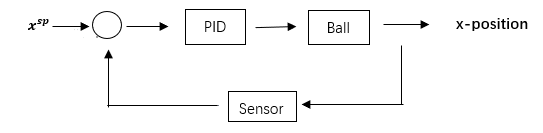
\includegraphics[width=1.0\linewidth]{Laser Sensor/All Control System.png}
        \caption{The complete control system }
    \end{minipage}
\end{figure}
    \section{Simulation}
Simulating the system allows the effect of the controller on the system to be analysed. It allows us to see the
outcome that different inputs will have on the system, including an impulse response and a step response.
The results from the simulation can be displayed on a graph. The PID values used were found via trial and error methods.
\subsection*{PID absent plots} \hfill \\
\begin{figure}[ht]
    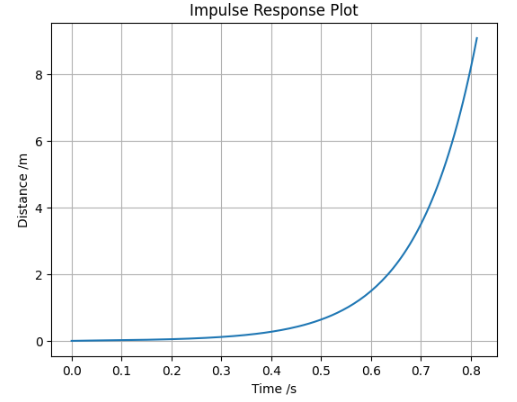
\includegraphics[width=0.65\linewidth]{Simulation/Impulse Plot no pid.png}
        \caption{Impulse response of the transfer function.}
\end{figure}

\begin{figure}[ht]
    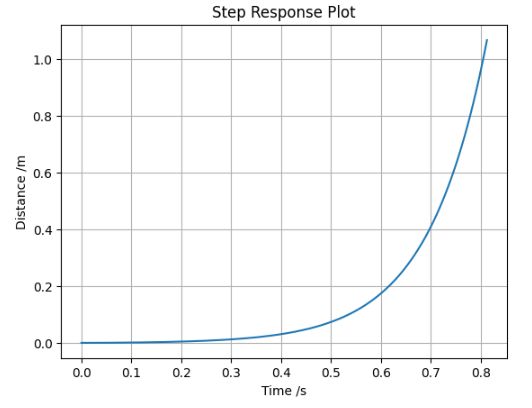
\includegraphics[width=0.65\linewidth]{Simulation/Step Plot no pid.png}
    \caption{Step response of the transfer function.}
\end{figure}

\noindent According to the Figure of the impulse response of the transfer function, When an instantaneous impact is applied to the system, the ball starts to move down the inclined plane  with increasing speed and acceleration. From the Figure of Step response of the transfer function, its situation is similar to the previous one, but with slower speed and acceleration. This illustrates the instability of a system without a controller.
\subsection*{PID plots}\hfill \\
\noindent The PID values chosen for this controller are Kp = 1135, Kd = 22.5, and Ki = 0. From the Figure of the impulse and step responses of the system, the line of impulse responses shows that the ball will move down the inclined plane between 0 and 0.1s and then upwards to a position 0.05mm from the equilibrium position. The step of impulse responses shows that when a constant force is applied to the system, the ball will move down the inclined plane and stabilise at a distance of 2.1mm from the equilibrium position. Therefore, the system is BIBO
stable, and it can be seen that the controller has a good control effect.
\begin{figure}[ht]
    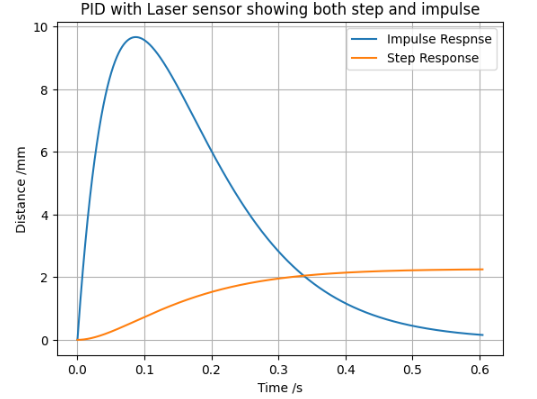
\includegraphics[width=0.65\linewidth]{Simulation/PID + Laser Both Step and Impulse plot.png}
    \caption{The impulse and step responses of the system.}
\end{figure}








    
\section{Team Collaboration}
\subsection*{Technologies}
\hfill \\
Discord was used to discuss the assignment, share each member’s progress, and discuss meeting times and locations. VS Code and Google Collaboratory were used to write the Python script, and Github was used to share the code. 
\subsection*{Management}\hfill \\
All members worked on completing the task of finding the transfer function. After that, tasks involving writing the code and the report were divided across the team. These tasks were managed well by each member and completed well on time.
\begin{figure}[ht]
    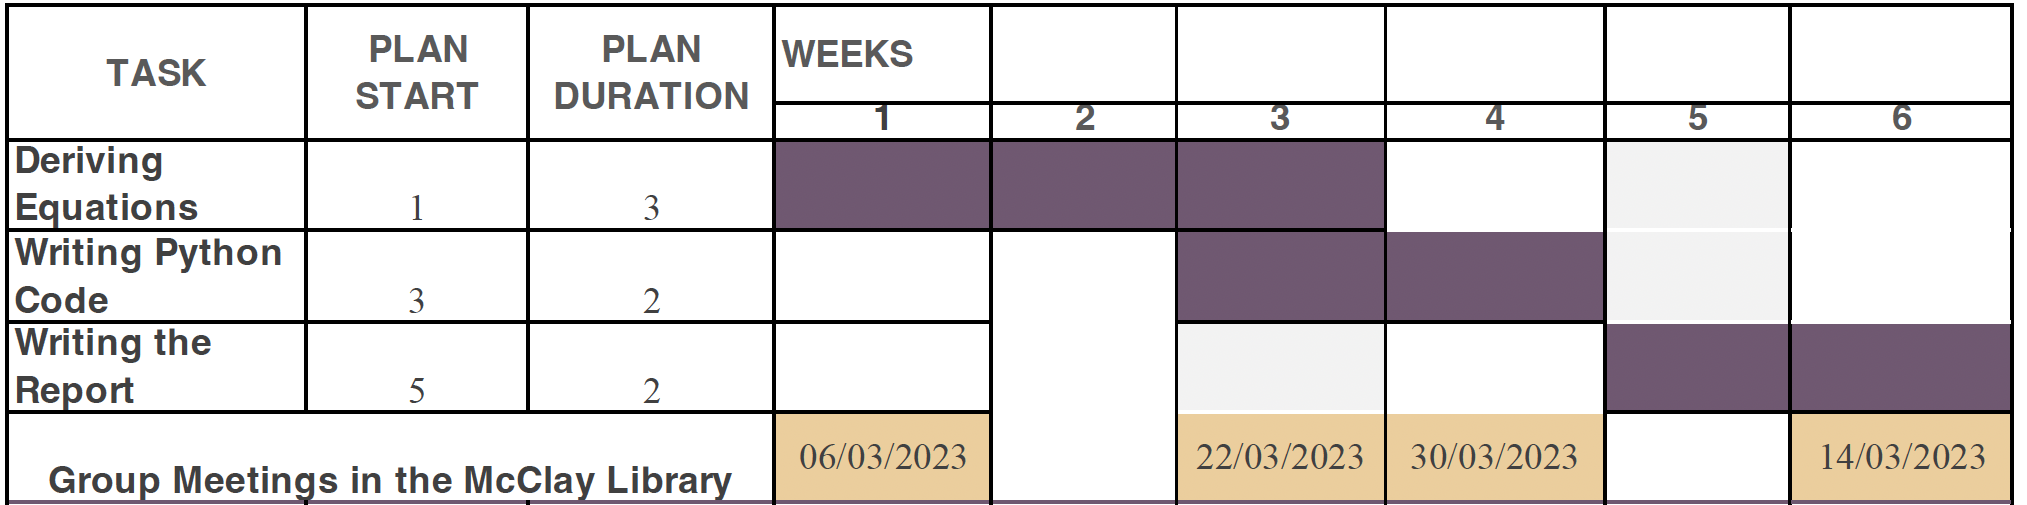
\includegraphics[width=0.8\linewidth]{Team collaboration/Screenshot 2023-04-16 at 19.28.44.png}
    \caption{Gantt chart of time management for coursework}
\end{figure}
\subsection*{Challenges}\hfill \\
Deriving the transfer function was a big challenge we faced and spent most of our time on.  
Choosing the PID values became a challenge as we tried to find the values that gave the best output. The values were decided using trial and error until we found values that we found to be good 
\subsection*{Contributions}\hfill \\
Each team member individually worked on deriving the equations and shared their progress with the other team members for them to compare and check the results.
\\
The tasks involving Python were divided as follows:
\begin{itemize}
  \item Michael Loughran worked on writing the code and the LaTeX for the equations, including the modelling of the system and the transfer function.
  \item Xiaohan Song worked on writing the code and the LaTeX for the simulations of the controller.
  \item Scott McNeilly worked on writing the bulk of the report and combining the sections of the other team members into one final report.
\end{itemize}

    \section*{Conclusion}
In conclusion, this is the working design for the controller we came up with. It fits the system requirements, being BIBO stable, having zero offset, avoiding large amplitude oscillations, and it rejects disturbances and holding the ball close to the set point and can bring the ball back to near the set point quickly when it is pushed or pulled.

\end{document}